\documentclass{article}

\usepackage[a4paper,top=2cm,bottom=2cm,left=3cm,right=3cm,marginparwidth=1.75cm]{geometry}
\usepackage[ngerman]{babel}
\usepackage{graphicx}
\usepackage{hyperref}
\usepackage{float}
\usepackage{color}

\title{ERA Übungsaufgaben W22/23}
\author{David Erb}
\begin{document}
\maketitle

\section{Einführung}
Dieses Aufgabenblatt wurde von Studenten erstellt, um zusätzliche Aufgaben für die Klausurvorbereitung bereitzustellen. Somit kann nicht für die Relevanz der Aufgaben im Bezug auf die Klausur bzw. für korrekte Lösungsvorschläge garantiert werden.

\section{Aufgaben}

\subsection{Aufgabe 1}
Einige Pinguine an der PUM sind Workaholics und machen viele Fehler, wenn sie zu lange am Stück arbeiten. Daher hat ein Pinguin eine Ampelschaltung  entworfen, welche den Workaholics anzeigen soll, wann sie eine Pause machen sollen. Die Schaltung hat 4 Zustände: Grün(Startzustand), Gelb, Rot und Pause. Jedes Mal wenn ein Pinguin einen Fehler(Input = 1) macht, soll sich der Zustand der Ampel um eins verschlechtern. Von Rot gerät man dabei in den Pause-Zustand, den man bei keiner der Input-Werte verlässt. Macht der Pinguin bei einer Aufgabe keinen Fehler(Input = 0), während die Schaltung nicht im Pause-Zustand ist, schaltet die Ampel wieder auf grün. Die Ampel ist also im Pause-Zustand wenn der Pinguin irgendwann einmal drei Fehler in Folge gemacht hat. Nur in dem Pause-Zustand soll die Ampel dem Pinguin das Signal geben, eine Pause zu machen (Output = 1)
(\hyperref[sec:lsg01]{Lösungsvorschlag}). \\
\\
i) Zeichne den Moore-Automat dieser Schaltung.\\
\\
ii) Fülle die Wahrheitstabelle der Zustandsübergangsfunktion des Automaten aus. Die Zustände haben folgende Binärkodierung: \\
Grün: 00 \\
Gelb: 01 \\
Rot: 10 \\
Pause 11 \\
\texttt{FFn} ist dabei das \texttt{n}te Bit des Zustands und \texttt{FFn'} das jeweilige Bit des Folgezustands.\\
I ist der Input, O der Output.\\ 
\\
\begin{tabular}{c|c|c|c|c|c|c}
   I  & FF1 & FF0 & FF1' & FF0' & O \\
    \hline
   0   &  0   & 0   &      &      &   \\
    \hline
   0  &   0  &  1   &      &      &   \\
     \hline
   0  &  1   &  0   &      &      &   \\
     \hline
   0  &   1  &  1   &      &      &   \\
     \hline
   1  &  0   &  0   &      &      &   \\
     \hline
   1  &   0  &  1   &      &      &   \\
     \hline
   1  &  1   &  0   &      &      &   \\
     \hline
   1  &  1   &   1  &      &      &   \\
     \hline
\end{tabular} \\
\\
iii) Gib den boolschen Term von \texttt{FF0'} an.

\subsection{Aufgabe 2}
Die Pinguine dürfen zu ihrer DS-Klausur leider keinen Taschenrechner mitnehmen. Da Pinguin Eric nicht besonders gut im Kopfrechnen ist ihm die Berechnung der Formel $n^k$ aus der Kombinatorik besonders schwerfällt, schreibt er ein rekursives Assemblerprogramm welches er während der Klausur ausführen, und damit schummeln kann. Jedoch hat er kurz nach Fertigstellung Kaffee über seinem Programm verschüttet!!
Hilf ihm, die entstandenen Lücken zu ersetzen.
Folgende Register sollen danach unverändert sein:
EAX, EBX, ECX, EDX, ESI, EDI, EBP, ESP (\hyperref[sec:lsg02]{Lösungsvorschlag}).
\begin{verbatim}
power_rec:
    ; 1. Stackparameter: k
    ; 2. Stackparameter: n
    ; 3. Stackparameter: Platz für den Rückgabewert
    ______
    MOV EBP, ESP
    PUSH EAX
    PUSH EBX
    MOV EAX, [EBP + 8]
    CMP EAX, 0
    ______
    MOV EBX, [EBP + 12]
    DEC ___
    SUB ESP, 4
    PUSH EBX
    PUSH EAX
    call power_rec
    ADD ESP, 8
    POP EAX
    ______
    MOV [EBP + 16], EAX
    JMP end
power_ret:
    MOV ______
end:
    ______
    ______
    ______
    ret
\end{verbatim}

\newpage

\section{Lösungsvorschläge}

\subsection{Aufgabe 1 (Lösungsvorschlag)}
i)
\begin{figure}[H]
\centering
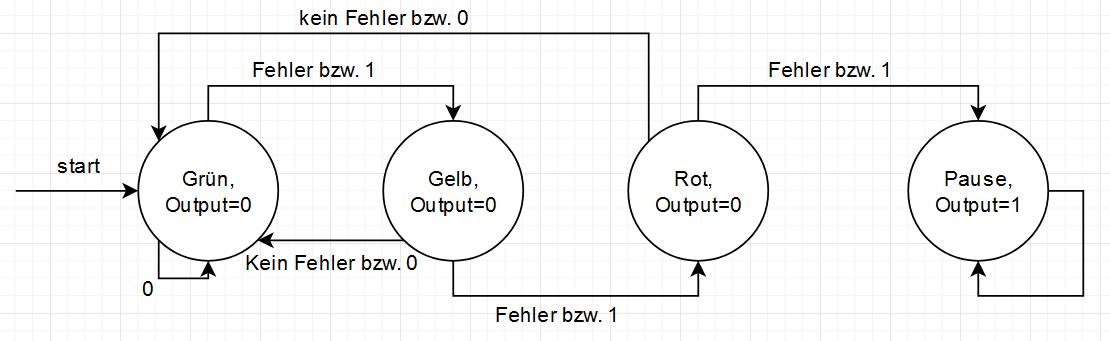
\includegraphics[scale=0.45]{automat.png}
\caption{Moore-Automat der Ampelschaltung}
\end{figure}

ii) \\
\\
\begin{tabular}{c|c|c|c|c|c|c}
   I  & FF1 & FF0 & FF1' & FF0' & O \\
    \hline
   0   &  0   & 0   &   0   &   0   & 0  \\
    \hline
   0  &   0  &  1   &  0    &   0   &  0 \\
     \hline
   0  &  1   &  0   &   0   &   0   & 0  \\
     \hline
   0  &   1  &  1   &   1   &   1   & 1  \\
     \hline
   1  &  0   &  0   &   0   &   1   &  0 \\
     \hline
   1  &   0  &  1   &   1   &   0   &  0 \\
     \hline
   1  &  1   &  0   &   1   &   1   & 0  \\
     \hline
   1  &  1   &   1  &   1   &   1   &  1 \\
     \hline
\end{tabular} \\
 \\
iii) \\
\\
\texttt{FF0' = FF1 FF0 + I $\neg FF0$}
\label{sec:lsg01}

\subsection{Aufgabe 2 (Lösungsvorschlag)}
\begin{verbatim}
power_rec:
    ; 1. Stackparameter: n
    ; 2. Stackparameter: x
    ; 3. Stackparameter: Platz für den Rückgabewert
    PUSH EBP
    MOV EBP, ESP
    PUSH EAX
    PUSH EBX
    MOV EAX, [EBP + 8]
    CMP EAX, 0
    JE power_ret
    MOV EBX, [EBP + 12]
    DEC EAX
    SUB ESP, 4
    PUSH EBX
    PUSH EAX
    call power_rec
    ADD ESP, 8
    POP EAX
    MUL EBX
    MOV [EBP + 16], EAX
    JMP end
power_ret:
    MOV [EPB + 16], 1
end:
    POP EAX
    POP EBX
    POP EBP
    ret
\end{verbatim}
\label{sec:lsg02}
\end{document}
